% Figure: maximum likelihood and the variational free energy are one statement
% read in two coordinate systems.  Design width ~168mm.
\documentclass[border=0pt]{standalone}
\usepackage{amsmath,amssymb}
% Shared visual language for the figures of the book.
% Every figure in this directory loads this file so the chapter reads as one system.
% NOTE: no blank lines are allowed inside \tikzset{...} (a blank line emits \par
% and breaks key scanning).
\NeedsTeXFormat{LaTeX2e}
\ProvidesPackage{figstyle}[2026/10/21 Figure style for Free Energy to LLMs]

\RequirePackage{tikz}
\usetikzlibrary{arrows.meta,positioning,calc,fit,shapes.geometric,shapes.misc,%
  backgrounds,matrix,decorations.pathreplacing,decorations.markings,patterns.meta}

% ---------------------------------------------------------------- palette
% Same values as book/preamble/style.tex, prefixed with F.
\definecolor{FNavy}{HTML}{14324A}
\definecolor{FTeal}{HTML}{0E7490}
\definecolor{FSky}{HTML}{E7F5F8}
\definecolor{FOrange}{HTML}{D97706}
\definecolor{FAmber}{HTML}{FFF3D6}
\definecolor{FInk}{HTML}{1F2937}
\definecolor{FSlate}{HTML}{64748B}
\definecolor{FMist}{HTML}{F5F7FA}
\definecolor{FRose}{HTML}{9F1239}
\definecolor{FRoseMist}{HTML}{FFF1F2}

% ---------------------------------------------------------------- semantics
% Teal   = probability / model / data object
% Orange = training objective, cost, or the quantity moved through the system
% Navy   = neutral structure
% Slate  = secondary label or metadata
% Rose   = failure mode, hazard, masked-out region
\tikzset{
  % Lay figures out in millimetres.  A figure designed 168mm wide is included at
  % \textwidth, so its fonts appear at exactly the size written here.
  every picture/.style={x=1mm,y=1mm,font=\small,line cap=round,line join=round},
  % ---- block styles
  nbase/.style={draw,rounded corners=1.2pt,align=center,inner sep=2.4pt,%
    minimum height=7mm,text=FInk},
  nteal/.style={nbase,draw=FTeal,fill=FSky},
  norange/.style={nbase,draw=FOrange,fill=FAmber},
  nnavy/.style={nbase,draw=FNavy,fill=white},
  nsoft/.style={nbase,draw=FSlate!55,fill=FMist},
  nrose/.style={nbase,draw=FRose,fill=FRoseMist},
  ghost/.style={draw=none,fill=none,align=center,inner sep=1pt},
  plain/.style={draw=none,fill=none,align=center,inner sep=0pt},
  % ---- arrows
  ar/.style={-{Latex[length=1.7mm,width=1.35mm]},draw=FSlate,line width=0.75pt},
  ard/.style={ar,dashed},
  arteal/.style={ar,draw=FTeal},
  arorange/.style={ar,draw=FOrange},
  arrose/.style={ar,draw=FRose},
  thickar/.style={ar,line width=1.2pt},
  % ---- text roles
  ftitle/.style={font=\large\bfseries,text=FNavy,align=center},
  ptitle/.style={font=\small\bfseries,text=FNavy,align=center},
  ptitleo/.style={font=\small\bfseries,text=FOrange,align=center},
  lbl/.style={font=\scriptsize,text=FSlate,align=center,inner sep=1pt},
  lblt/.style={lbl,text=FTeal},
  lblo/.style={lbl,text=FOrange},
  lbln/.style={lbl,text=FNavy},
  lblr/.style={lbl,text=FRose},
  sub/.style={font=\scriptsize,text=FSlate!90,align=center,inner sep=1pt},
  monob/.style={font=\ttfamily\scriptsize,text=FInk,inner sep=1pt},
  mathb/.style={font=\small,text=FInk,inner sep=1pt},
  eqn/.style={font=\scriptsize,inner sep=1.5pt,text=FInk},
  % ---- decorations
  brace/.style={decorate,decoration={brace,amplitude=2.4pt},draw=FSlate,%
    line width=0.6pt},
  bracet/.style={brace,draw=FTeal},
  braceo/.style={brace,draw=FOrange},
  axis/.style={draw=FSlate!55,line width=0.6pt},
  guide/.style={draw=FSlate!45,line width=0.5pt,dashed},
  halolabel/.style={font=\scriptsize,text=FInk,fill=white,fill opacity=0.85,%
    text opacity=1,inner sep=1.4pt,align=center},
}

% Figure title above the drawing, anchored at the figure's top-left.
\newcommand{\figtitle}[2][0]{%
  \node[ftitle,anchor=north west,outer sep=0pt] at (#1,0) {#2};}

% Rounded panel behind a subgroup of nodes.
\newcommand{\figpanel}[3][]{%
  \node[draw=FSlate!35,fill=#3,rounded corners=2pt,inner sep=2.6mm,#1] {#2};}

\endinput

\begin{document}
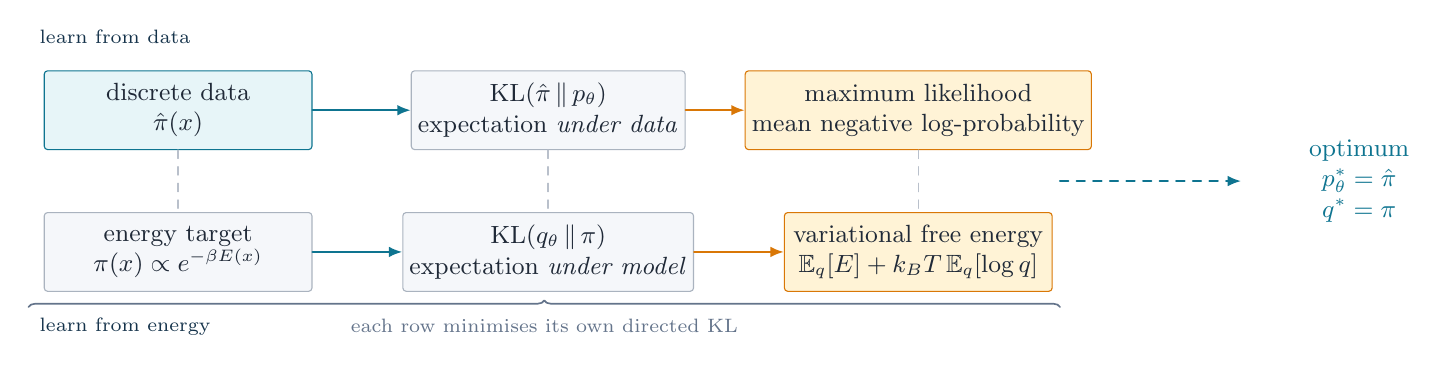
\begin{tikzpicture}
\node[nteal,minimum width=34mm,minimum height=10mm] (data) at (0,9)
  {discrete data\\$\hat\pi(x)$};
\node[nsoft,minimum width=34mm,minimum height=10mm] (kl1) at (47,9)
  {$\mathrm{KL}(\hat\pi\,\Vert\,p_\theta)$\\expectation \emph{under data}};
\node[norange,minimum width=34mm,minimum height=10mm] (mle) at (94,9)
  {maximum likelihood\\mean negative log-probability};

\node[nsoft,minimum width=34mm,minimum height=10mm] (energy) at (0,-9)
  {energy target\\$\pi(x)\propto e^{-\beta E(x)}$};
\node[nsoft,minimum width=34mm,minimum height=10mm] (kl2) at (47,-9)
  {$\mathrm{KL}(q_\theta\,\Vert\,\pi)$\\expectation \emph{under model}};
\node[norange,minimum width=34mm,minimum height=10mm] (free) at (94,-9)
  {variational free energy\\$\mathbb{E}_q[E]+k_BT\,\mathbb{E}_q[\log q]$};

\draw[arteal] (data)--(kl1);
\draw[arorange] (kl1)--(mle);
\draw[arteal] (energy)--(kl2);
\draw[arorange] (kl2)--(free);

% the two rows differ only in which distribution the expectation is taken over
\draw[guide] (data.south)--(energy.north);
\draw[guide] (kl1.south)--(kl2.north);
\draw[guide] (mle.south)--(free.north);

\node[lbln,anchor=south west] at (-18,17) {learn from data};
\node[lbln,anchor=north west] at (-18,-17){learn from energy};

\draw[brace] (-19,-16)--(112,-16)
  node[midway,below=3pt,lbl]
  {each row minimises its own directed KL};

\node[plain,font=\small,text=FTeal] at (150,0) {optimum\\$p_\theta^*=\hat\pi$\\$q^*=\pi$};
\draw[arteal,dashed] (112,0)--(135,0);
\end{tikzpicture}
\end{document}
